\documentclass{article}
\usepackage{amsmath}
\usepackage{amssymb}
\usepackage{fullpage}
\usepackage[parfill]{parskip}
\usepackage{pythonhighlight}
\usepackage{scrextend}
\usepackage{tikz}
\newcommand{\pd}[2]{\frac{\partial #1}{\partial #2}}
\title{Assignment 2 writeup}
\author{Thomas Lu}
\date{}
\begin{document}
\maketitle
\section{Problem 1}
(c) Placeholders are nodes in a TF computation graph whose values are populated at runtime. These nodes are often used to populate training data. Feed dictionaries, meanwhile, are what actually do the populating at runtime; they specify at runtime a mapping of placeholder nodes to actual values.

(e) When \pyth{train_op} is called, we compute during forward propagation (for a batch) predictions $\hat{y} = \text{softmax}(xW + b)$ and the loss $J = CE(y, \hat{y})$, where $CE$ denotes cross-entropy loss. Then we compute during backpropagation the partial gradients $\partial J/\partial W$ and $\partial J/\partial b$ and add a negative multiple of these gradients to our variables $W$ and $b$.

\section{Problem 2}
(a)
\begin{center}
\footnotesize
\begin{tabular}{l|l|l|l}
stack & buffer & new dependency & transition\\
\hline
{[ROOT]} & [I, parsed, this, sentence, correctly] & & Initial Configuration \\
{[ROOT, I]} & [parsed, this, sentence, correctly] & & SHIFT \\
{[ROOT, I, parsed]} & [this, sentence, correctly] & & SHIFT \\
{[ROOT, parsed]} & [this, sentence, correctly] & parsed $\rightarrow$ I & LEFT-ARC \\
{[ROOT, parsed, this]} & [sentence, correctly] & & SHIFT \\
{[ROOT, parsed, this, sentence]} & [correctly] & & SHIFT \\
{[ROOT, parsed, sentence]} & [correctly] & sentence $\rightarrow$ this & LEFT-ARC \\
{[ROOT, parsed]} & [correctly] & parsed $\rightarrow$ sentence & RIGHT-ARC \\
{[ROOT, parsed, correctly]} & [] & & SHIFT \\
{[ROOT, parsed]} & [] & parsed $\rightarrow$ correctly & RIGHT-ARC \\
{[ROOT]} & [] & ROOT $\rightarrow$ parsed & RIGHT-ARC \\
\end{tabular}
\end{center}

(b) A written sentence of $n$ words will require $2n$ steps: each word requires one step to move it from the buffer to the stack, and one to move it from the stack to the dependency tree.

(f) We have
$$ h_i = \mathbb{E}_{drop}[h_{drop}]_i = \gamma (1 - p_{drop}) h_i,$$
so $\gamma = 1/(1 - p_{drop})$.

(g)
\begin{itemize}
\item (i) Momentum basically slows the rate at which we adjust our updates: instead of immediately updating using the current gradient, we instead continue mostly going in the direction of our previous momentum and only assign a partial influence to the current gradient on our next update. This can help us avoid large ``bad" updates when we see a particularly anomalous batch of training data or when we hit a particularly steep gradient wall.
\item (ii) Adam amplifies the movement of parameters with small gradient contributions and reduces that of parameters with large gradient contributions. This can help in cases where we might have large almost-flat regions and small steep walls in our gradient function.
\end{itemize}

(h) The best dev UAS was 88.71, and the tes UAS was 89.19.

\section{Problem 3}
(a)

(i) Suppose that $y^{(t)} = w \in V$. We have
\begin{align*}
CE^{(t)}\left(y^{(t)}, \hat{y}^{(t)}\right) &= -\sum_{j=1}^{|V|} y_j^{(t)}\log \hat{y}_j^{(t)} = -\log \hat{y}_w^{(t)}\\
PP^{(t)}\left(y^{(t)}, \hat{y}^{(t)}\right) &= \frac{1}{\sum_{j=1}^{|V|} y_j^{(t)}\hat{y}_j^{(t)}} = \frac{1}{\hat{y}_w^{(t)}}\\
&= e^{CE^{(t)}\left(y^{(t)}, \hat{y}^{(t)}\right)}
\end{align*}

(ii) We have
\begin{align*}
\left(\prod_{t=1}^T PP\left(y^{(t)}, \hat{y}^{(t)}\right)\right)^{1/T} &= \left(\prod_{t=1}^T e^{CE\left(y^{(t)}, \hat{y}^{(t)}\right)}\right)^{1/T} \\
&= e^{(1/T)\sum_{t=1}^T CE\left(y^{(t)}, \hat{y}^{(t)}\right)} \\,
\end{align*}
from which it is clear that the geometric mean of perplexity and the arithmetic mean of cross-entropy are equivalent objectives.

(iii) The perplexity would be $1/\hat{y}_w^{(t)} = 1/(1/|V|) = |V|$, where $w$ denotes the correct word. For $V$ = 10000, the cross-entropy is
$$\log PP\left(y^{(t)}, \hat{y}^{(t)}\right) = \log 10000 \approx 9.2103.$$

(b)

Let $\theta^{(t)} = Uh^{(t)} + b_2,$ so that $\hat{y}^{(t)} = \text{softmax}(\theta^{(t)})$. Suppose that $y^{(t)}$ is one-hot at $w_t$. We then have
\begin{align*}
\pd{J^{(t)}}{\theta^{(t)}} &= \pd{}{\theta^{(t)}_j} - \log \frac{e^{\theta^{(t)}_{w_t}}}{\sum_{j=1}^{|V|} e^{\theta^{(t)}}_j} \\
&= - \left( \pd{}{\theta^{(t)}}\log e^{\theta^{(t)}_{w_t}} - \pd{}{\theta^{(t)}} \log\left(\sum_{j=1}^{|V|} e^{\theta^{(t)}_j}\right) \right) \\
&= - \left( \pd{}{\theta^{(t)}} \theta^{(t)}_{w_t} - \frac{\pd{}{\theta^{(t)}} \sum_{j=1}^{|V|} e^{\theta^{(t)}_j}}{\sum_{j=1}^{|V|} e^{\theta^{(t)}_j}}\right) \\
&= \text{softmax}(\theta^{(t)}) - y^{(t)}.
\end{align*}
Let
$$\delta_1^{(t)} = \pd{J^{(t)}}{\theta^{(t)}} = \text{softmax}(\theta^{(t)}) - y^{(t)}.$$
Then
$$\pd{J^{(t)}}{U} = \pd{J^{(t)}}{\theta^{(t)}} \pd{\theta^{(t)}}{U} = \delta_1^{(t)} \pd{\theta^{(t)}}{U}.$$
We have
$$\pd{\theta^{(t)}}{U_{ij}} = h^{(t)}_j1_i,$$
where $1_i$ denotes the one-hot vector (of equal dimension as $\theta^{(t)}$) with 1 at position $i$. This implies
\begin{align*}
\pd{J^{(t)}}{U_{ij}} &= \left(\pd{J^{(t)}}{\theta^{(t)}}\right)^T \pd{\theta^{(t)}}{U_{ij}}\\
&= h^{(t)}_j\left(\text{softmax}(\theta^{(t)}) - y^{(t)}\right)_i \\
\Rightarrow \pd{J^{(t)}}{U} &= \left(\text{softmax}(\theta^{(t)}) - y^{(t)}\right) \left(h^{(t)}\right)^T\\
&= \delta_1^{(t)} \left(h^{(t)}\right)^T.
\end{align*}
Now let $z^{(t)} = W_h h^{(t-1)} + W_e e^{(t)} + b_1$, so that $h^{(t)} = \sigma(z^{(t)}).$ It is easy to see that
\begin{align*}
\pd{J^{(t)}}{e^{(t)}} &= \left(\pd{z^{(t)}}{e^{(t)}}\right)^T \pd{J^{(t)}}{z^{(t)}} = W_e^T\delta_2^{(t)} \\
\left. \pd{J^{(t)}}{W_e} \right|_{(t)} &= \left(\left.\pd{z^{(t)}}{W_e}\right|_{(t)}\right)^T \pd{J^{(t)}}{z^{(t)}} = \delta_2^{(t)}(e^{(t)})^T \\
\left. \pd{J^{(t)}}{W_h}\right|_{(t)} &= \left(\left.\pd{z^{(t)}}{W_h}\right|_{(t)}\right)^T \pd{J^{(t)}}{z^{(t)}} = \delta_2^{(t)}(h^{(t-1)})^T \\
\pd{J^{(t)}}{h^{(t-1)}} &= \left(\pd{z^{(t)}}{h^{(t-1)}}\right)^T \pd{J^{(t)}}{z^{(t)}} = W_h^T\delta_2^{(t)}
\end{align*}
where
$$\delta_2^{(t)} = \pd{J^{(t)}}{z^{(t)}}$$
and
$$\pd{v}{A}$$
for a vector $v$ and matrix $A$ denotes a vector $v'$ of matrices $v_1', v_2', \dots, v_n'$ with 
$$v_k' = \pd{v_k}{A}.$$
It suffices to compute $\delta_2^{(t)}.$ We have
\begin{align*}
\delta_2^{(t)} &= \pd{J^{(t)}}{z^{(t)}} = \left( \pd{\theta^{(t)}}{h^{(t)}} \pd{h^{(t)}}{z^{(t)}}\right)^T \pd{J^{(t)}}{\theta^{(t)}} \\
&= \left(U \text{diag}\left(\sigma(z^{(t)} \circ (1 - \sigma(z^{(t)})) \right)\right)^T \delta_1^{(t)}\\
&= h^{(t)} \circ \left(1 - h^{(t)}\right) \circ \left(U^T\delta_1^{(t)}\right)
\end{align*}

(c)
\begin{figure}
\centering
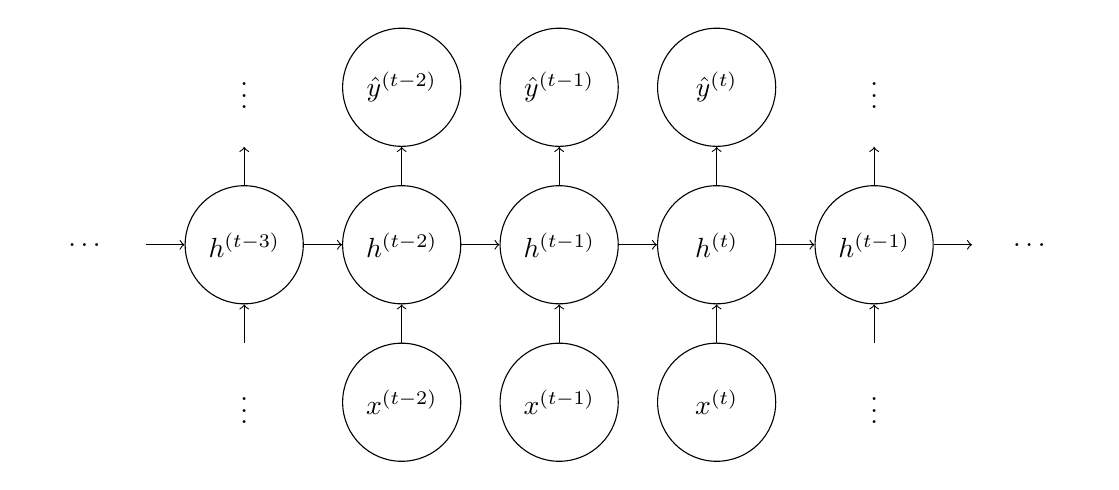
\begin{tikzpicture}[
    rnnstep/.style={shape=circle, draw=black, minimum size=1.5cm},
    rnnempty/.style={shape=circle, draw opacity=0, minimum size=1.5cm},
]
\node[rnnempty] (hm3) at (0, 2) {$\dots$};
\node[rnnempty] (xm2) at (2, 0) {$\vdots$};
\node[rnnempty] (ym2) at (2, 4) {$\vdots$};
\node[rnnstep] (hm2) at (2, 2) {$h^{(t-3)}$};
\node[rnnstep] (ym1) at (4, 4) {$\hat{y}^{(t-2)}$};
\node[rnnstep] (xm1) at (4, 0) {$x^{(t-2)}$};
\node[rnnstep] (hm1) at (4, 2) {$h^{(t-2)}$};
\node[rnnstep] (h0) at (6, 2) {$h^{(t-1)}$};
\node[rnnstep] (y0) at (6, 4) {$\hat{y}^{(t-1)}$};
\node[rnnstep] (x0) at (6, 0) {$x^{(t-1)}$};
\node[rnnstep] (h1) at (8, 2) {$h^{(t)}$};
\node[rnnstep] (y1) at (8, 4) {$\hat{y}^{(t)}$};
\node[rnnstep] (x1) at (8, 0) {$x^{(t)}$};
\node[rnnstep] (h2) at (10, 2) {$h^{(t-1)}$};
\node[rnnempty] (x2) at (10, 0) {$\vdots$};
\node[rnnempty] (y2) at (10, 4) {$\vdots$};
\node[rnnempty] (h3) at (12, 2) {$\dots$};

\path[->]
    (hm3) edge node {} (hm2)
    (xm2) edge node {} (hm2)
    (hm2) edge node {} (ym2)
    (hm2) edge node {} (hm1)
    (xm1) edge node {} (hm1)
    (hm1) edge node {} (ym1)
    (hm1) edge node {} (h0)
    (x0) edge node {} (h0)
    (h0) edge node {} (y0)
    (h0) edge node {} (h1)
    (h1) edge node {} (y1)
    (x1) edge node {} (h1)
    (h1) edge node {} (h2)
    (h2) edge node {} (y2)
    (x2) edge node {} (h2)
    (h2) edge node {} (h3)
;
\end{tikzpicture}
\caption{The RNN unrolled to 3 steps.} \label{fig3c}
\end{figure}
Figure \ref{fig3c} depicts the unrolled RNN.

We have
\begin{align*}
\pd{J^{(t)}}{e^{(t-1)}} &= \left(\pd{h^{(t-1)}}{e^{(t-1)}}\right)^T \pd{J^{(t)}}{h^{(t-1)}}\\
&= \left(\pd{h^{(t-1)}}{z^{(t-1)}} \pd{z^{(t-1)}}{e^{(t-1)}} \right)^T \gamma^{(t-1)}\\ 
&= W_e^T \left( h^{(t-1)} \circ (1 - h^{(t-1)}) \circ \gamma^{(t-1)}\right),
\end{align*}
where $\gamma^{(t-1)} = \partial J^{(t)} / \partial h^{(t-1)}.$ Similarly,
\begin{align*}
\left.\pd{J^{(t)}}{W_e}\right|_{(t-1)} &= \left(\left. \pd{z^{(t-1)}}{W_e}\right|_{(t-1)} \right)^T \pd{J^{(t)}}{z^{(t-1)}} \\
&= \left(\left. \pd{z^{(t-1)}}{W_e}\right|_{(t-1)} \right)^T \left(h^{(t-1)} \circ (1 - h^{(t-1)}) \circ \gamma^{(t-1)}\right) \\
&= \left(h^{(t-1)} \circ (1 - h^{(t-1)}) \circ \gamma^{(t-1)}\right) (e^{(t-1)})^T\\
\left.\pd{J^{(t)}}{W_h}\right|_{(t-1)} &= \left(\left. \pd{z^{(t-1)}}{W_h}\right|_{(t-1)} \right)^T \pd{J^{(t)}}{z^{(t-1)}} \\
&= \left(\left. \pd{z^{(t-1)}}{W_h}\right|_{(t-1)} \right)^T \left(h^{(t-1)} \circ (1 - h^{(t-1)}) \circ \gamma^{(t-1)}\right) \\
&= \left(h^{(t-1)} \circ (1 - h^{(t-1)}) \circ \gamma^{(t-1)}\right) (h^{(t-2)})^T.\\
\end{align*}

(d)

\begin{itemize}
\item Computing $\partial J^{(t)} / \partial U$ requires constructing a $|V| \times D_h$ matrix, so will require $|V|D_h$ operations.
\item Computing $\delta_2$, which is needed in the computations of $\partial J^{(t)} / \partial e^{(t)}$, $\partial J^{(t)} / \partial W_e |_{(t)}$, $\partial J^{(t)} / \partial W_h |_{(t)}$, and $\partial J^{(t)} / \partial h^{(t-1)}$, requires multiplying a $D_h \times |V|$ matrix by a vector of length $|V|$, so it requires $|V|D_h$ operations. $\delta_2$ is a vector of length $D_h$.
\item Computing $\partial J^{(t)} / \partial e^{(t)}$ requires multiplying a $d \times D_h$ matrix by a vector of length $D_h$, so it takes $dD_h$ operations.
\item Computing $\partial J^{(t)} / \partial W_e |_{(t)}$ requires constructing a $D_h \times d$ matrix, so requires $dD_h$ operations.
\item Computing $\partial J^{(t)} / \partial W_h |_{(t)}$ requires constructing a $D_h \times D_h$ matrix, so requires $D_h^2$ operations.
\item Computing $\partial J^{(t)} / \partial h^{(t-1)}$ requires multiplying a $D_h \times D_h$ matrix by a vector of length $D_h$, so requires $D_h^2$ operations.
\end{itemize}
Thus computing the gradients for one time step requires $O(|V|D_h + dD_h + D_h^2)$ operations.

(e)

If we compute the gradients for the time steps in reverse chronological order, we only have to pass error signals from one time step to the previous one once for each time step. Then computing the gradients for all time steps for a sequence of words of length $T$ requires $O(T(|V|D_h + dD_h + D_h^2))$ operations.

(f)

The largest term in the big-$O$ estimate is likely to be $|V|D_h$, which comes from the output layer of the RNN.
\end{document}
